\documentclass[1p]{elsarticle_modified}
%\bibliographystyle{elsarticle-num}

%\usepackage[colorlinks]{hyperref}
%\usepackage{abbrmath_seonhwa} %\Abb, \Ascr, \Acal ,\Abf, \Afrak
\usepackage{amsfonts}
\usepackage{amssymb}
\usepackage{amsmath}
\usepackage{amsthm}
\usepackage{scalefnt}
\usepackage{amsbsy}
\usepackage{kotex}
\usepackage{caption}
\usepackage{subfig}
\usepackage{color}
\usepackage{graphicx}
\usepackage{xcolor} %% white, black, red, green, blue, cyan, magenta, yellow
\usepackage{float}
\usepackage{setspace}
\usepackage{hyperref}

\usepackage{tikz}
\usetikzlibrary{arrows}

\usepackage{multirow}
\usepackage{array} % fixed length table
\usepackage{hhline}

%%%%%%%%%%%%%%%%%%%%%
\makeatletter
\renewcommand*\env@matrix[1][\arraystretch]{%
	\edef\arraystretch{#1}%
	\hskip -\arraycolsep
	\let\@ifnextchar\new@ifnextchar
	\array{*\c@MaxMatrixCols c}}
\makeatother %https://tex.stackexchange.com/questions/14071/how-can-i-increase-the-line-spacing-in-a-matrix
%%%%%%%%%%%%%%%

\usepackage[normalem]{ulem}

\newcommand{\msout}[1]{\ifmmode\text{\sout{\ensuremath{#1}}}\else\sout{#1}\fi}
%SOURCE: \msout is \stkout macro in https://tex.stackexchange.com/questions/20609/strikeout-in-math-mode

\newcommand{\cancel}[1]{
	\ifmmode
	{\color{red}\msout{#1}}
	\else
	{\color{red}\sout{#1}}
	\fi
}

\newcommand{\add}[1]{
	{\color{blue}\uwave{#1}}
}

\newcommand{\replace}[2]{
	\ifmmode
	{\color{red}\msout{#1}}{\color{blue}\uwave{#2}}
	\else
	{\color{red}\sout{#1}}{\color{blue}\uwave{#2}}
	\fi
}

\newcommand{\Sol}{\mathcal{S}} %segment
\newcommand{\D}{D} %diagram
\newcommand{\A}{\mathcal{A}} %arc


%%%%%%%%%%%%%%%%%%%%%%%%%%%%%5 test

\def\sl{\operatorname{\textup{SL}}(2,\Cbb)}
\def\psl{\operatorname{\textup{PSL}}(2,\Cbb)}
\def\quan{\mkern 1mu \triangleright \mkern 1mu}

\theoremstyle{definition}
\newtheorem{thm}{Theorem}[section]
\newtheorem{prop}[thm]{Proposition}
\newtheorem{lem}[thm]{Lemma}
\newtheorem{ques}[thm]{Question}
\newtheorem{cor}[thm]{Corollary}
\newtheorem{defn}[thm]{Definition}
\newtheorem{exam}[thm]{Example}
\newtheorem{rmk}[thm]{Remark}
\newtheorem{alg}[thm]{Algorithm}

\newcommand{\I}{\sqrt{-1}}
\begin{document}

%\begin{frontmatter}
%
%\title{Boundary parabolic representations of knots up to 8 crossings}
%
%%% Group authors per affiliation:
%\author{Yunhi Cho} 
%\address{Department of Mathematics, University of Seoul, Seoul, Korea}
%\ead{yhcho@uos.ac.kr}
%
%
%\author{Seonhwa Kim} %\fnref{s_kim}}
%\address{Center for Geometry and Physics, Institute for Basic Science, Pohang, 37673, Korea}
%\ead{ryeona17@ibs.re.kr}
%
%\author{Hyuk Kim}
%\address{Department of Mathematical Sciences, Seoul National University, Seoul 08826, Korea}
%\ead{hyukkim@snu.ac.kr}
%
%\author{Seokbeom Yoon}
%\address{Department of Mathematical Sciences, Seoul National University, Seoul, 08826,  Korea}
%\ead{sbyoon15@snu.ac.kr}
%
%\begin{abstract}
%We find all boundary parabolic representation of knots up to 8 crossings.
%
%\end{abstract}
%\begin{keyword}
%    \MSC[2010] 57M25 
%\end{keyword}
%
%\end{frontmatter}

%\linenumbers
%\tableofcontents
%
\newcommand\colored[1]{\textcolor{white}{\rule[-0.35ex]{0.8em}{1.4ex}}\kern-0.8em\color{red} #1}%
%\newcommand\colored[1]{\textcolor{white}{ #1}\kern-2.17ex	\textcolor{white}{ #1}\kern-1.81ex	\textcolor{white}{ #1}\kern-2.15ex\color{red}#1	}

{\Large $\underline{12a_{0839}~(K12a_{0839})}$}

\setlength{\tabcolsep}{10pt}
\renewcommand{\arraystretch}{1.6}
\vspace{1cm}\begin{tabular}{m{100pt}>{\centering\arraybackslash}m{274pt}}
\multirow{5}{120pt}{
	\centering
	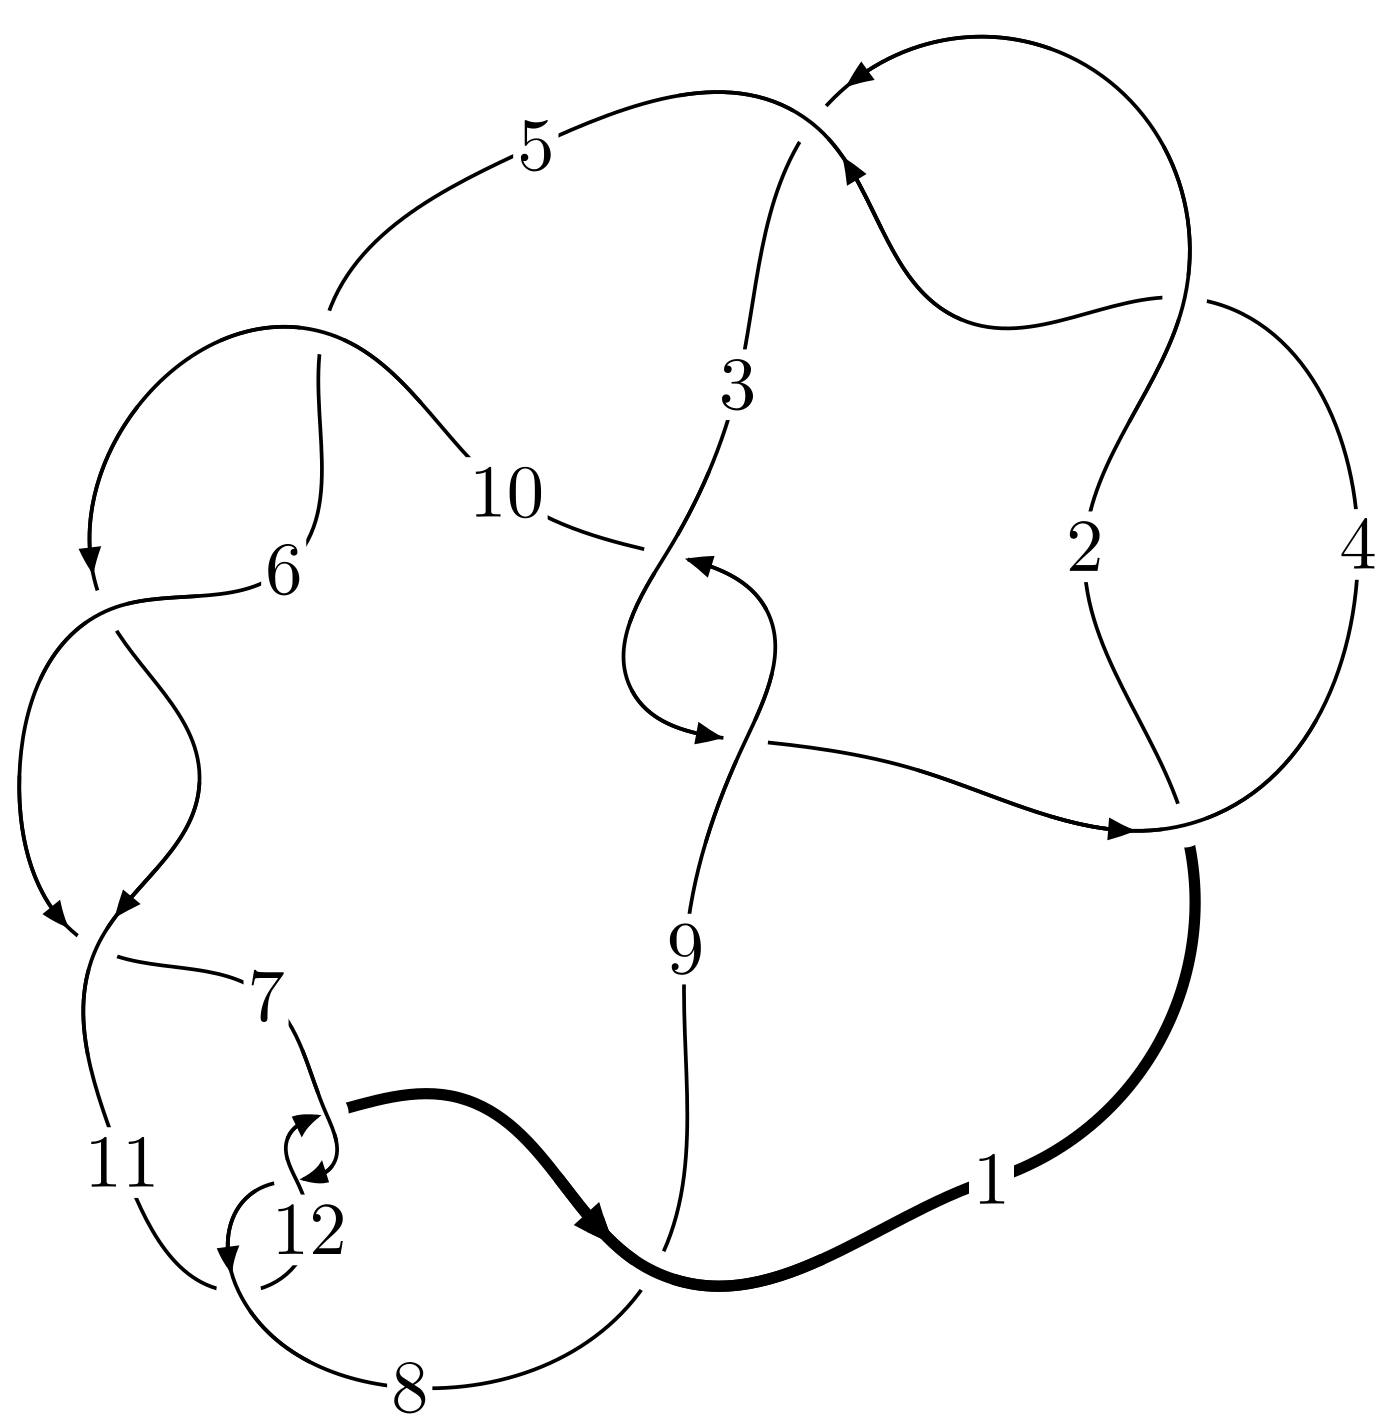
\includegraphics[width=112pt]{../../../GIT/diagram.site/Diagrams/png/1640_12a_0839.png}\\
\ \ \ A knot diagram\footnotemark}&
\allowdisplaybreaks
\textbf{Linearized knot diagam} \\
\cline{2-2}
 &
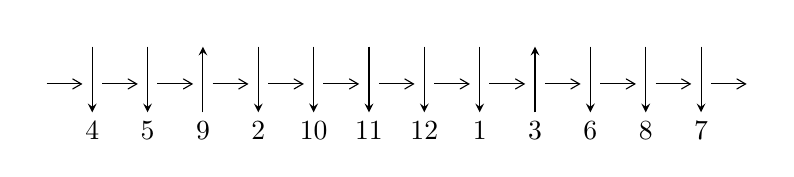
\begin{tikzpicture}[x=20pt, y=17pt]
	% nodes
	\node (C0) at (0, 0) {};
	\node (C1) at (1, 0) {};
	\node (C1U) at (1, +1) {};
	\node (C1D) at (1, -1) {4};

	\node (C2) at (2, 0) {};
	\node (C2U) at (2, +1) {};
	\node (C2D) at (2, -1) {5};

	\node (C3) at (3, 0) {};
	\node (C3U) at (3, +1) {};
	\node (C3D) at (3, -1) {9};

	\node (C4) at (4, 0) {};
	\node (C4U) at (4, +1) {};
	\node (C4D) at (4, -1) {2};

	\node (C5) at (5, 0) {};
	\node (C5U) at (5, +1) {};
	\node (C5D) at (5, -1) {10};

	\node (C6) at (6, 0) {};
	\node (C6U) at (6, +1) {};
	\node (C6D) at (6, -1) {11};

	\node (C7) at (7, 0) {};
	\node (C7U) at (7, +1) {};
	\node (C7D) at (7, -1) {12};

	\node (C8) at (8, 0) {};
	\node (C8U) at (8, +1) {};
	\node (C8D) at (8, -1) {1};

	\node (C9) at (9, 0) {};
	\node (C9U) at (9, +1) {};
	\node (C9D) at (9, -1) {3};

	\node (C10) at (10, 0) {};
	\node (C10U) at (10, +1) {};
	\node (C10D) at (10, -1) {6};

	\node (C11) at (11, 0) {};
	\node (C11U) at (11, +1) {};
	\node (C11D) at (11, -1) {8};

	\node (C12) at (12, 0) {};
	\node (C12U) at (12, +1) {};
	\node (C12D) at (12, -1) {7};
	\node (C13) at (13, 0) {};

	% arrows
	\draw[->,>={angle 60}]
	(C0) edge (C1) (C1) edge (C2) (C2) edge (C3) (C3) edge (C4) (C4) edge (C5) (C5) edge (C6) (C6) edge (C7) (C7) edge (C8) (C8) edge (C9) (C9) edge (C10) (C10) edge (C11) (C11) edge (C12) (C12) edge (C13) ;	\draw[->,>=stealth]
	(C1U) edge (C1D) (C2U) edge (C2D) (C3D) edge (C3U) (C4U) edge (C4D) (C5U) edge (C5D) (C6U) edge (C6D) (C7U) edge (C7D) (C8U) edge (C8D) (C9D) edge (C9U) (C10U) edge (C10D) (C11U) edge (C11D) (C12U) edge (C12D) ;
	\end{tikzpicture} \\
\hhline{~~} \\& 
\textbf{Solving Sequence} \\ \cline{2-2} 
 &
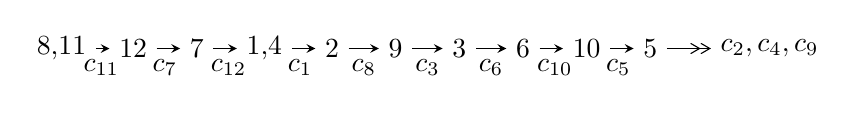
\begin{tikzpicture}[x=23pt, y=7pt]
	% node
	\node (A0) at (-1/8, 0) {8,11};
	\node (A1) at (1, 0) {12};
	\node (A2) at (2, 0) {7};
	\node (A3) at (49/16, 0) {1,4};
	\node (A4) at (33/8, 0) {2};
	\node (A5) at (41/8, 0) {9};
	\node (A6) at (49/8, 0) {3};
	\node (A7) at (57/8, 0) {6};
	\node (A8) at (65/8, 0) {10};
	\node (A9) at (73/8, 0) {5};
	\node (C1) at (1/2, -1) {$c_{11}$};
	\node (C2) at (3/2, -1) {$c_{7}$};
	\node (C3) at (5/2, -1) {$c_{12}$};
	\node (C4) at (29/8, -1) {$c_{1}$};
	\node (C5) at (37/8, -1) {$c_{8}$};
	\node (C6) at (45/8, -1) {$c_{3}$};
	\node (C7) at (53/8, -1) {$c_{6}$};
	\node (C8) at (61/8, -1) {$c_{10}$};
	\node (C9) at (69/8, -1) {$c_{5}$};
	\node (A10) at (11, 0) {$c_{2},c_{4},c_{9}$};

	% edge
	\draw[->,>=stealth]	
	(A0) edge (A1) (A1) edge (A2) (A2) edge (A3) (A3) edge (A4) (A4) edge (A5) (A5) edge (A6) (A6) edge (A7) (A7) edge (A8) (A8) edge (A9) ;
	\draw[->>,>={angle 60}]	
	(A9) edge (A10);
\end{tikzpicture} \\ 

\end{tabular} \\

\footnotetext{
The image of knot diagram is generated by the software ``\textbf{Draw programme}" developed by Andrew Bartholomew(\url{http://www.layer8.co.uk/maths/draw/index.htm\#Running-draw}), where we modified some parts for our purpose(\url{https://github.com/CATsTAILs/LinksPainter}).
}\phantom \\ \newline 
\centering \textbf{Ideals for irreducible components\footnotemark of $X_{\text{par}}$} 
 
\begin{align*}
I^u_{1}&=\langle 
u^{42}+u^{41}+\cdots+b+u,\;- u^{28}-11 u^{26}+\cdots+a-1,\;u^{47}+2 u^{46}+\cdots-2 u-1\rangle \\
I^u_{2}&=\langle 
u^3+b+u,\;u^2+a+1,\;u^6- u^5+3 u^4-2 u^3+2 u^2- u-1\rangle \\
\\
\end{align*}
\raggedright * 2 irreducible components of $\dim_{\mathbb{C}}=0$, with total 53 representations.\\
\footnotetext{All coefficients of polynomials are rational numbers. But the coefficients are sometimes approximated in decimal forms when there is not enough margin.}
\newpage
\renewcommand{\arraystretch}{1}
\centering \section*{I. $I^u_{1}= \langle u^{42}+u^{41}+\cdots+b+u,\;- u^{28}-11 u^{26}+\cdots+a-1,\;u^{47}+2 u^{46}+\cdots-2 u-1 \rangle$}
\flushleft \textbf{(i) Arc colorings}\\
\begin{tabular}{m{7pt} m{180pt} m{7pt} m{180pt} }
\flushright $a_{8}=$&$\begin{pmatrix}0\\u\end{pmatrix}$ \\
\flushright $a_{11}=$&$\begin{pmatrix}1\\0\end{pmatrix}$ \\
\flushright $a_{12}=$&$\begin{pmatrix}1\\u^2\end{pmatrix}$ \\
\flushright $a_{7}=$&$\begin{pmatrix}u\\u^3+u\end{pmatrix}$ \\
\flushright $a_{1}=$&$\begin{pmatrix}u^2+1\\u^4+2 u^2\end{pmatrix}$ \\
\flushright $a_{4}=$&$\begin{pmatrix}u^{28}+11 u^{26}+\cdots+8 u+1\\- u^{42}- u^{41}+\cdots-9 u^2- u\end{pmatrix}$ \\
\flushright $a_{2}=$&$\begin{pmatrix}- u^{46}- u^{45}+\cdots-11 u^2-6 u\\- u^{46}-2 u^{45}+\cdots+3 u+1\end{pmatrix}$ \\
\flushright $a_{9}=$&$\begin{pmatrix}- u^5-2 u^3- u\\- u^7-3 u^5-2 u^3+u\end{pmatrix}$ \\
\flushright $a_{3}=$&$\begin{pmatrix}2 u^{46}+2 u^{45}+\cdots+14 u^2+7 u\\2 u^{46}+4 u^{45}+\cdots-4 u-2\end{pmatrix}$ \\
\flushright $a_{6}=$&$\begin{pmatrix}u^3+2 u\\u^3+u\end{pmatrix}$ \\
\flushright $a_{10}=$&$\begin{pmatrix}- u^6-3 u^4-2 u^2+1\\- u^6-2 u^4- u^2\end{pmatrix}$ \\
\flushright $a_{5}=$&$\begin{pmatrix}- u^9-4 u^7-5 u^5+3 u\\- u^9-3 u^7-3 u^5+u\end{pmatrix}$\\&\end{tabular}
\flushleft \textbf{(ii) Obstruction class $= -1$}\\~\\
\flushleft \textbf{(iii) Cusp Shapes $= 4 u^{46}+8 u^{45}+\cdots+8 u-13$}\\~\\
\newpage\renewcommand{\arraystretch}{1}
\flushleft \textbf{(iv) u-Polynomials at the component}\newline \\
\begin{tabular}{m{50pt}|m{274pt}}
Crossings & \hspace{64pt}u-Polynomials at each crossing \\
\hline $$\begin{aligned}c_{1},c_{2},c_{4}\end{aligned}$$&$\begin{aligned}
&u^{47}-7 u^{46}+\cdots-7 u+1
\end{aligned}$\\
\hline $$\begin{aligned}c_{3},c_{9}\end{aligned}$$&$\begin{aligned}
&u^{47}- u^{46}+\cdots+128 u+64
\end{aligned}$\\
\hline $$\begin{aligned}c_{5},c_{6},c_{8}\\c_{10}\end{aligned}$$&$\begin{aligned}
&u^{47}-2 u^{46}+\cdots-18 u-9
\end{aligned}$\\
\hline $$\begin{aligned}c_{7},c_{11},c_{12}\end{aligned}$$&$\begin{aligned}
&u^{47}+2 u^{46}+\cdots-2 u-1
\end{aligned}$\\
\hline
\end{tabular}\\~\\
\newpage\renewcommand{\arraystretch}{1}
\flushleft \textbf{(v) Riley Polynomials at the component}\newline \\
\begin{tabular}{m{50pt}|m{274pt}}
Crossings & \hspace{64pt}Riley Polynomials at each crossing \\
\hline $$\begin{aligned}c_{1},c_{2},c_{4}\end{aligned}$$&$\begin{aligned}
&y^{47}-51 y^{46}+\cdots+47 y-1
\end{aligned}$\\
\hline $$\begin{aligned}c_{3},c_{9}\end{aligned}$$&$\begin{aligned}
&y^{47}+39 y^{46}+\cdots+36864 y-4096
\end{aligned}$\\
\hline $$\begin{aligned}c_{5},c_{6},c_{8}\\c_{10}\end{aligned}$$&$\begin{aligned}
&y^{47}-60 y^{46}+\cdots+1494 y-81
\end{aligned}$\\
\hline $$\begin{aligned}c_{7},c_{11},c_{12}\end{aligned}$$&$\begin{aligned}
&y^{47}+36 y^{46}+\cdots+22 y-1
\end{aligned}$\\
\hline
\end{tabular}\\~\\
\newpage\flushleft \textbf{(vi) Complex Volumes and Cusp Shapes}
$$\begin{array}{c|c|c}  
\text{Solutions to }I^u_{1}& \I (\text{vol} + \sqrt{-1}CS) & \text{Cusp shape}\\
 \hline 
\begin{aligned}
u &= -0.931573 + 0.033964 I \\
a &= -3.62555 - 1.06085 I \\
b &= -4.04479 - 1.25290 I\end{aligned}
 & \phantom{-}18.8163 + 7.6066 I & -17.4102 - 3.4010 I \\ \hline\begin{aligned}
u &= -0.931573 - 0.033964 I \\
a &= -3.62555 + 1.06085 I \\
b &= -4.04479 + 1.25290 I\end{aligned}
 & \phantom{-}18.8163 - 7.6066 I & -17.4102 + 3.4010 I \\ \hline\begin{aligned}
u &= \phantom{-}0.925379\phantom{ +0.000000I} \\
a &= \phantom{-}4.48125\phantom{ +0.000000I} \\
b &= \phantom{-}5.06824\phantom{ +0.000000I}\end{aligned}
 & -15.5609\phantom{ +0.000000I} & -16.5480\phantom{ +0.000000I} \\ \hline\begin{aligned}
u &= -0.921953 + 0.011274 I \\
a &= \phantom{-}1.352420 - 0.172739 I \\
b &= \phantom{-}1.42411 + 0.22950 I\end{aligned}
 & -13.30020 + 3.04123 I & -15.7591 - 2.6303 I \\ \hline\begin{aligned}
u &= -0.921953 - 0.011274 I \\
a &= \phantom{-}1.352420 + 0.172739 I \\
b &= \phantom{-}1.42411 - 0.22950 I\end{aligned}
 & -13.30020 - 3.04123 I & -15.7591 + 2.6303 I \\ \hline\begin{aligned}
u &= \phantom{-}0.350823 + 1.049320 I \\
a &= \phantom{-}1.24839 - 0.95940 I \\
b &= \phantom{-}1.86804 + 0.49348 I\end{aligned}
 & -8.18690 + 1.30928 I & -14.5225 + 0. I\phantom{ +0.000000I} \\ \hline\begin{aligned}
u &= \phantom{-}0.350823 - 1.049320 I \\
a &= \phantom{-}1.24839 + 0.95940 I \\
b &= \phantom{-}1.86804 - 0.49348 I\end{aligned}
 & -8.18690 - 1.30928 I & -14.5225 + 0. I\phantom{ +0.000000I} \\ \hline\begin{aligned}
u &= \phantom{-}0.885281\phantom{ +0.000000I} \\
a &= -1.61021\phantom{ +0.000000I} \\
b &= -1.68165\phantom{ +0.000000I}\end{aligned}
 & -8.45625\phantom{ +0.000000I} & -8.69640\phantom{ +0.000000I} \\ \hline\begin{aligned}
u &= \phantom{-}0.044109 + 1.177400 I \\
a &= -0.897270 + 0.427390 I \\
b &= \phantom{-}0.26502 + 1.43818 I\end{aligned}
 & \phantom{-}1.19605 - 0.94580 I & -9.30810 + 0. I\phantom{ +0.000000I} \\ \hline\begin{aligned}
u &= \phantom{-}0.044109 - 1.177400 I \\
a &= -0.897270 - 0.427390 I \\
b &= \phantom{-}0.26502 - 1.43818 I\end{aligned}
 & \phantom{-}1.19605 + 0.94580 I & -9.30810 + 0. I\phantom{ +0.000000I}\\
 \hline 
 \end{array}$$\newpage$$\begin{array}{c|c|c}  
\text{Solutions to }I^u_{1}& \I (\text{vol} + \sqrt{-1}CS) & \text{Cusp shape}\\
 \hline 
\begin{aligned}
u &= \phantom{-}0.262817 + 1.164060 I \\
a &= -0.677836 + 0.380418 I \\
b &= \phantom{-}0.236782 - 0.642439 I\end{aligned}
 & -0.606425 - 1.119520 I & -12.48597 + 0. I\phantom{ +0.000000I} \\ \hline\begin{aligned}
u &= \phantom{-}0.262817 - 1.164060 I \\
a &= -0.677836 - 0.380418 I \\
b &= \phantom{-}0.236782 + 0.642439 I\end{aligned}
 & -0.606425 + 1.119520 I & -12.48597 + 0. I\phantom{ +0.000000I} \\ \hline\begin{aligned}
u &= -0.173486 + 1.230470 I \\
a &= \phantom{-}0.394455 + 0.372411 I \\
b &= \phantom{-}0.781097 + 0.132649 I\end{aligned}
 & \phantom{-}2.76219 + 2.33868 I & \phantom{-0.000000 } 0 \\ \hline\begin{aligned}
u &= -0.173486 - 1.230470 I \\
a &= \phantom{-}0.394455 - 0.372411 I \\
b &= \phantom{-}0.781097 - 0.132649 I\end{aligned}
 & \phantom{-}2.76219 - 2.33868 I & \phantom{-0.000000 } 0 \\ \hline\begin{aligned}
u &= -0.283890 + 1.214980 I \\
a &= -0.93375 - 1.68089 I \\
b &= -2.46189 - 0.25027 I\end{aligned}
 & -2.16231 + 3.49023 I & \phantom{-0.000000 } 0 \\ \hline\begin{aligned}
u &= -0.283890 - 1.214980 I \\
a &= -0.93375 + 1.68089 I \\
b &= -2.46189 + 0.25027 I\end{aligned}
 & -2.16231 - 3.49023 I & \phantom{-0.000000 } 0 \\ \hline\begin{aligned}
u &= \phantom{-}0.729642 + 0.166193 I \\
a &= -2.35770 + 1.36778 I \\
b &= -1.47388 + 0.31386 I\end{aligned}
 & -10.80020 - 5.29604 I & -17.2800 + 4.5994 I \\ \hline\begin{aligned}
u &= \phantom{-}0.729642 - 0.166193 I \\
a &= -2.35770 - 1.36778 I \\
b &= -1.47388 - 0.31386 I\end{aligned}
 & -10.80020 + 5.29604 I & -17.2800 - 4.5994 I \\ \hline\begin{aligned}
u &= -0.057596 + 1.253360 I \\
a &= \phantom{-}0.339761 - 0.116633 I \\
b &= \phantom{-}0.339456 - 1.125610 I\end{aligned}
 & \phantom{-}3.89474 + 1.72506 I & \phantom{-0.000000 } 0 \\ \hline\begin{aligned}
u &= -0.057596 - 1.253360 I \\
a &= \phantom{-}0.339761 + 0.116633 I \\
b &= \phantom{-}0.339456 + 1.125610 I\end{aligned}
 & \phantom{-}3.89474 - 1.72506 I & \phantom{-0.000000 } 0\\
 \hline 
 \end{array}$$\newpage$$\begin{array}{c|c|c}  
\text{Solutions to }I^u_{1}& \I (\text{vol} + \sqrt{-1}CS) & \text{Cusp shape}\\
 \hline 
\begin{aligned}
u &= \phantom{-}0.271270 + 1.256580 I \\
a &= \phantom{-}0.044945 + 0.350451 I \\
b &= -0.929623 + 1.047440 I\end{aligned}
 & \phantom{-}0.20223 - 5.63538 I & \phantom{-0.000000 } 0 \\ \hline\begin{aligned}
u &= \phantom{-}0.271270 - 1.256580 I \\
a &= \phantom{-}0.044945 - 0.350451 I \\
b &= -0.929623 - 1.047440 I\end{aligned}
 & \phantom{-}0.20223 + 5.63538 I & \phantom{-0.000000 } 0 \\ \hline\begin{aligned}
u &= -0.681129\phantom{ +0.000000I} \\
a &= \phantom{-}3.55601\phantom{ +0.000000I} \\
b &= \phantom{-}1.84966\phantom{ +0.000000I}\end{aligned}
 & -5.84226\phantom{ +0.000000I} & -16.3910\phantom{ +0.000000I} \\ \hline\begin{aligned}
u &= \phantom{-}0.663598 + 0.066636 I \\
a &= \phantom{-}0.818243 - 0.611101 I \\
b &= \phantom{-}0.281216 - 0.780752 I\end{aligned}
 & -3.85427 - 2.27055 I & -16.0301 + 4.5719 I \\ \hline\begin{aligned}
u &= \phantom{-}0.663598 - 0.066636 I \\
a &= \phantom{-}0.818243 + 0.611101 I \\
b &= \phantom{-}0.281216 + 0.780752 I\end{aligned}
 & -3.85427 + 2.27055 I & -16.0301 - 4.5719 I \\ \hline\begin{aligned}
u &= \phantom{-}0.418616 + 1.278440 I \\
a &= \phantom{-}0.422426 - 0.961243 I \\
b &= \phantom{-}1.59423 + 0.48650 I\end{aligned}
 & -4.48545 - 4.66586 I & \phantom{-0.000000 } 0 \\ \hline\begin{aligned}
u &= \phantom{-}0.418616 - 1.278440 I \\
a &= \phantom{-}0.422426 + 0.961243 I \\
b &= \phantom{-}1.59423 - 0.48650 I\end{aligned}
 & -4.48545 + 4.66586 I & \phantom{-0.000000 } 0 \\ \hline\begin{aligned}
u &= -0.098317 + 1.342180 I \\
a &= \phantom{-}0.247608 + 0.502928 I \\
b &= -1.198420 + 0.642791 I\end{aligned}
 & -1.25656 + 3.25255 I & \phantom{-0.000000 } 0 \\ \hline\begin{aligned}
u &= -0.098317 - 1.342180 I \\
a &= \phantom{-}0.247608 - 0.502928 I \\
b &= -1.198420 - 0.642791 I\end{aligned}
 & -1.25656 - 3.25255 I & \phantom{-0.000000 } 0 \\ \hline\begin{aligned}
u &= -0.467449 + 1.264530 I \\
a &= \phantom{-}1.55167 + 2.04635 I \\
b &= \phantom{-}3.15396 - 2.12723 I\end{aligned}
 & -16.8558 - 2.6238 I & \phantom{-0.000000 } 0\\
 \hline 
 \end{array}$$\newpage$$\begin{array}{c|c|c}  
\text{Solutions to }I^u_{1}& \I (\text{vol} + \sqrt{-1}CS) & \text{Cusp shape}\\
 \hline 
\begin{aligned}
u &= -0.467449 - 1.264530 I \\
a &= \phantom{-}1.55167 - 2.04635 I \\
b &= \phantom{-}3.15396 + 2.12723 I\end{aligned}
 & -16.8558 + 2.6238 I & \phantom{-0.000000 } 0 \\ \hline\begin{aligned}
u &= \phantom{-}0.290224 + 1.319350 I \\
a &= \phantom{-}0.22664 - 1.55655 I \\
b &= \phantom{-}1.55061 - 0.91105 I\end{aligned}
 & -6.15563 - 8.92874 I & \phantom{-0.000000 } 0 \\ \hline\begin{aligned}
u &= \phantom{-}0.290224 - 1.319350 I \\
a &= \phantom{-}0.22664 + 1.55655 I \\
b &= \phantom{-}1.55061 + 0.91105 I\end{aligned}
 & -6.15563 + 8.92874 I & \phantom{-0.000000 } 0 \\ \hline\begin{aligned}
u &= -0.450761 + 1.279910 I \\
a &= -0.262410 - 0.919173 I \\
b &= -0.848073 + 0.408862 I\end{aligned}
 & -9.36462 + 1.85590 I & \phantom{-0.000000 } 0 \\ \hline\begin{aligned}
u &= -0.450761 - 1.279910 I \\
a &= -0.262410 + 0.919173 I \\
b &= -0.848073 - 0.408862 I\end{aligned}
 & -9.36462 - 1.85590 I & \phantom{-0.000000 } 0 \\ \hline\begin{aligned}
u &= \phantom{-}0.449749 + 1.289880 I \\
a &= -1.11666 + 2.79890 I \\
b &= -4.69994 - 1.43155 I\end{aligned}
 & -11.55410 - 4.90637 I & \phantom{-0.000000 } 0 \\ \hline\begin{aligned}
u &= \phantom{-}0.449749 - 1.289880 I \\
a &= -1.11666 - 2.79890 I \\
b &= -4.69994 + 1.43155 I\end{aligned}
 & -11.55410 + 4.90637 I & \phantom{-0.000000 } 0 \\ \hline\begin{aligned}
u &= -0.430024 + 0.463380 I \\
a &= \phantom{-}0.073435 - 0.954770 I \\
b &= \phantom{-}0.627166 + 0.371706 I\end{aligned}
 & -6.80327 + 1.66591 I & -14.4251 - 3.8260 I \\ \hline\begin{aligned}
u &= -0.430024 - 0.463380 I \\
a &= \phantom{-}0.073435 + 0.954770 I \\
b &= \phantom{-}0.627166 - 0.371706 I\end{aligned}
 & -6.80327 - 1.66591 I & -14.4251 + 3.8260 I \\ \hline\begin{aligned}
u &= -0.443644 + 1.297270 I \\
a &= -0.442064 - 0.748189 I \\
b &= -1.82872 + 0.23677 I\end{aligned}
 & -9.23009 + 7.91648 I & \phantom{-0.000000 } 0\\
 \hline 
 \end{array}$$\newpage$$\begin{array}{c|c|c}  
\text{Solutions to }I^u_{1}& \I (\text{vol} + \sqrt{-1}CS) & \text{Cusp shape}\\
 \hline 
\begin{aligned}
u &= -0.443644 - 1.297270 I \\
a &= -0.442064 + 0.748189 I \\
b &= -1.82872 - 0.23677 I\end{aligned}
 & -9.23009 - 7.91648 I & \phantom{-0.000000 } 0 \\ \hline\begin{aligned}
u &= -0.443422 + 1.315870 I \\
a &= \phantom{-}0.30539 + 2.51704 I \\
b &= \phantom{-}4.35921 + 0.13601 I\end{aligned}
 & -16.4532 + 12.5153 I & \phantom{-0.000000 } 0 \\ \hline\begin{aligned}
u &= -0.443422 - 1.315870 I \\
a &= \phantom{-}0.30539 - 2.51704 I \\
b &= \phantom{-}4.35921 - 0.13601 I\end{aligned}
 & -16.4532 - 12.5153 I & \phantom{-0.000000 } 0 \\ \hline\begin{aligned}
u &= -0.475692\phantom{ +0.000000I} \\
a &= -1.09705\phantom{ +0.000000I} \\
b &= -0.304127\phantom{ +0.000000I}\end{aligned}
 & -0.943106\phantom{ +0.000000I} & -10.1730\phantom{ +0.000000I} \\ \hline\begin{aligned}
u &= -0.220025 + 0.246765 I \\
a &= -0.83102 + 1.27964 I \\
b &= -0.099600 + 0.370710 I\end{aligned}
 & -0.433930 + 0.816857 I & -9.44363 - 8.26201 I \\ \hline\begin{aligned}
u &= -0.220025 - 0.246765 I \\
a &= -0.83102 - 1.27964 I \\
b &= -0.099600 - 0.370710 I\end{aligned}
 & -0.433930 - 0.816857 I & -9.44363 + 8.26201 I \\ \hline\begin{aligned}
u &= \phantom{-}0.228742\phantom{ +0.000000I} \\
a &= \phantom{-}2.90776\phantom{ +0.000000I} \\
b &= -0.724057\phantom{ +0.000000I}\end{aligned}
 & -2.00058\phantom{ +0.000000I} & \phantom{-}0.109480\phantom{ +0.000000I}\\
 \hline 
 \end{array}$$\newpage\newpage\renewcommand{\arraystretch}{1}
\centering \section*{II. $I^u_{2}= \langle u^3+b+u,\;u^2+a+1,\;u^6- u^5+3 u^4-2 u^3+2 u^2- u-1 \rangle$}
\flushleft \textbf{(i) Arc colorings}\\
\begin{tabular}{m{7pt} m{180pt} m{7pt} m{180pt} }
\flushright $a_{8}=$&$\begin{pmatrix}0\\u\end{pmatrix}$ \\
\flushright $a_{11}=$&$\begin{pmatrix}1\\0\end{pmatrix}$ \\
\flushright $a_{12}=$&$\begin{pmatrix}1\\u^2\end{pmatrix}$ \\
\flushright $a_{7}=$&$\begin{pmatrix}u\\u^3+u\end{pmatrix}$ \\
\flushright $a_{1}=$&$\begin{pmatrix}u^2+1\\u^4+2 u^2\end{pmatrix}$ \\
\flushright $a_{4}=$&$\begin{pmatrix}- u^2-1\\- u^3- u\end{pmatrix}$ \\
\flushright $a_{2}=$&$\begin{pmatrix}0\\u^4- u^3+2 u^2- u\end{pmatrix}$ \\
\flushright $a_{9}=$&$\begin{pmatrix}- u^5-2 u^3- u\\- u^5+u^4-2 u^3+u^2- u-1\end{pmatrix}$ \\
\flushright $a_{3}=$&$\begin{pmatrix}- u^2-1\\- u^3- u\end{pmatrix}$ \\
\flushright $a_{6}=$&$\begin{pmatrix}u^3+2 u\\u^3+u\end{pmatrix}$ \\
\flushright $a_{10}=$&$\begin{pmatrix}- u^5-2 u^3- u\\- u^5+u^4-2 u^3+u^2- u-1\end{pmatrix}$ \\
\flushright $a_{5}=$&$\begin{pmatrix}- u^2-1\\- u^4-2 u^2\end{pmatrix}$\\&\end{tabular}
\flushleft \textbf{(ii) Obstruction class $= 1$}\\~\\
\flushleft \textbf{(iii) Cusp Shapes $= -5 u^4+6 u^3-11 u^2+6 u-17$}\\~\\
\newpage\renewcommand{\arraystretch}{1}
\flushleft \textbf{(iv) u-Polynomials at the component}\newline \\
\begin{tabular}{m{50pt}|m{274pt}}
Crossings & \hspace{64pt}u-Polynomials at each crossing \\
\hline $$\begin{aligned}c_{1},c_{2}\end{aligned}$$&$\begin{aligned}
&(u-1)^6
\end{aligned}$\\
\hline $$\begin{aligned}c_{3},c_{9}\end{aligned}$$&$\begin{aligned}
&u^6
\end{aligned}$\\
\hline $$\begin{aligned}c_{4}\end{aligned}$$&$\begin{aligned}
&(u+1)^6
\end{aligned}$\\
\hline $$\begin{aligned}c_{5},c_{6},c_{8}\end{aligned}$$&$\begin{aligned}
&u^6- u^5-3 u^4+2 u^3+2 u^2+u-1
\end{aligned}$\\
\hline $$\begin{aligned}c_{7}\end{aligned}$$&$\begin{aligned}
&u^6+u^5+3 u^4+2 u^3+2 u^2+u-1
\end{aligned}$\\
\hline $$\begin{aligned}c_{10}\end{aligned}$$&$\begin{aligned}
&u^6+u^5-3 u^4-2 u^3+2 u^2- u-1
\end{aligned}$\\
\hline $$\begin{aligned}c_{11},c_{12}\end{aligned}$$&$\begin{aligned}
&u^6- u^5+3 u^4-2 u^3+2 u^2- u-1
\end{aligned}$\\
\hline
\end{tabular}\\~\\
\newpage\renewcommand{\arraystretch}{1}
\flushleft \textbf{(v) Riley Polynomials at the component}\newline \\
\begin{tabular}{m{50pt}|m{274pt}}
Crossings & \hspace{64pt}Riley Polynomials at each crossing \\
\hline $$\begin{aligned}c_{1},c_{2},c_{4}\end{aligned}$$&$\begin{aligned}
&(y-1)^6
\end{aligned}$\\
\hline $$\begin{aligned}c_{3},c_{9}\end{aligned}$$&$\begin{aligned}
&y^6
\end{aligned}$\\
\hline $$\begin{aligned}c_{5},c_{6},c_{8}\\c_{10}\end{aligned}$$&$\begin{aligned}
&y^6-7 y^5+17 y^4-16 y^3+6 y^2-5 y+1
\end{aligned}$\\
\hline $$\begin{aligned}c_{7},c_{11},c_{12}\end{aligned}$$&$\begin{aligned}
&y^6+5 y^5+9 y^4+4 y^3-6 y^2-5 y+1
\end{aligned}$\\
\hline
\end{tabular}\\~\\
\newpage\flushleft \textbf{(vi) Complex Volumes and Cusp Shapes}
$$\begin{array}{c|c|c}  
\text{Solutions to }I^u_{2}& \I (\text{vol} + \sqrt{-1}CS) & \text{Cusp shape}\\
 \hline 
\begin{aligned}
u &= \phantom{-}0.873214\phantom{ +0.000000I} \\
a &= -1.76250\phantom{ +0.000000I} \\
b &= -1.53904\phantom{ +0.000000I}\end{aligned}
 & -9.30502\phantom{ +0.000000I} & -19.0600\phantom{ +0.000000I} \\ \hline\begin{aligned}
u &= -0.138835 + 1.234450 I \\
a &= \phantom{-}0.504580 + 0.342767 I \\
b &= -0.493180 + 0.575288 I\end{aligned}
 & \phantom{-}1.31531 + 1.97241 I & -8.22189 - 4.83849 I \\ \hline\begin{aligned}
u &= -0.138835 - 1.234450 I \\
a &= \phantom{-}0.504580 - 0.342767 I \\
b &= -0.493180 - 0.575288 I\end{aligned}
 & \phantom{-}1.31531 - 1.97241 I & -8.22189 + 4.83849 I \\ \hline\begin{aligned}
u &= \phantom{-}0.408802 + 1.276380 I \\
a &= \phantom{-}0.462019 - 1.043570 I \\
b &= \phantom{-}1.52087 + 0.16310 I\end{aligned}
 & -5.34051 - 4.59213 I & -15.2853 + 2.7994 I \\ \hline\begin{aligned}
u &= \phantom{-}0.408802 - 1.276380 I \\
a &= \phantom{-}0.462019 + 1.043570 I \\
b &= \phantom{-}1.52087 - 0.16310 I\end{aligned}
 & -5.34051 + 4.59213 I & -15.2853 - 2.7994 I \\ \hline\begin{aligned}
u &= -0.413150\phantom{ +0.000000I} \\
a &= -1.17069\phantom{ +0.000000I} \\
b &= \phantom{-}0.483672\phantom{ +0.000000I}\end{aligned}
 & -2.38379\phantom{ +0.000000I} & -21.9250\phantom{ +0.000000I}\\
 \hline 
 \end{array}$$\newpage
\newpage\renewcommand{\arraystretch}{1}
\centering \section*{ III. u-Polynomials}
\begin{tabular}{m{50pt}|m{274pt}}
Crossings & \hspace{64pt}u-Polynomials at each crossing \\
\hline $$\begin{aligned}c_{1},c_{2}\end{aligned}$$&$\begin{aligned}
&((u-1)^6)(u^{47}-7 u^{46}+\cdots-7 u+1)
\end{aligned}$\\
\hline $$\begin{aligned}c_{3},c_{9}\end{aligned}$$&$\begin{aligned}
&u^6(u^{47}- u^{46}+\cdots+128 u+64)
\end{aligned}$\\
\hline $$\begin{aligned}c_{4}\end{aligned}$$&$\begin{aligned}
&((u+1)^6)(u^{47}-7 u^{46}+\cdots-7 u+1)
\end{aligned}$\\
\hline $$\begin{aligned}c_{5},c_{6},c_{8}\end{aligned}$$&$\begin{aligned}
&(u^6- u^5-3 u^4+2 u^3+2 u^2+u-1)(u^{47}-2 u^{46}+\cdots-18 u-9)
\end{aligned}$\\
\hline $$\begin{aligned}c_{7}\end{aligned}$$&$\begin{aligned}
&(u^6+u^5+3 u^4+2 u^3+2 u^2+u-1)(u^{47}+2 u^{46}+\cdots-2 u-1)
\end{aligned}$\\
\hline $$\begin{aligned}c_{10}\end{aligned}$$&$\begin{aligned}
&(u^6+u^5-3 u^4-2 u^3+2 u^2- u-1)(u^{47}-2 u^{46}+\cdots-18 u-9)
\end{aligned}$\\
\hline $$\begin{aligned}c_{11},c_{12}\end{aligned}$$&$\begin{aligned}
&(u^6- u^5+3 u^4-2 u^3+2 u^2- u-1)(u^{47}+2 u^{46}+\cdots-2 u-1)
\end{aligned}$\\
\hline
\end{tabular}\newpage\renewcommand{\arraystretch}{1}
\centering \section*{ IV. Riley Polynomials}
\begin{tabular}{m{50pt}|m{274pt}}
Crossings & \hspace{64pt}Riley Polynomials at each crossing \\
\hline $$\begin{aligned}c_{1},c_{2},c_{4}\end{aligned}$$&$\begin{aligned}
&((y-1)^6)(y^{47}-51 y^{46}+\cdots+47 y-1)
\end{aligned}$\\
\hline $$\begin{aligned}c_{3},c_{9}\end{aligned}$$&$\begin{aligned}
&y^6(y^{47}+39 y^{46}+\cdots+36864 y-4096)
\end{aligned}$\\
\hline $$\begin{aligned}c_{5},c_{6},c_{8}\\c_{10}\end{aligned}$$&$\begin{aligned}
&(y^6-7 y^5+17 y^4-16 y^3+6 y^2-5 y+1)\\
&\cdot(y^{47}-60 y^{46}+\cdots+1494 y-81)
\end{aligned}$\\
\hline $$\begin{aligned}c_{7},c_{11},c_{12}\end{aligned}$$&$\begin{aligned}
&(y^6+5 y^5+\cdots-5 y+1)(y^{47}+36 y^{46}+\cdots+22 y-1)
\end{aligned}$\\
\hline
\end{tabular}
\vskip 2pc
\end{document}